\documentclass[conference]{IEEEtran}

\usepackage{graphicx}
\usepackage{xcolor}
\usepackage{tikz}
\usepackage{pgfplots}
\usepackage{booktabs}
\usepackage{array}
\usepackage{multirow}
\usepackage{url}
\usepackage{amsmath}
\usetikzlibrary{arrows.meta, positioning, calc, backgrounds}
\pgfplotsset{compat=1.18}

% System architecture diagram palette
\definecolor{cinput}{HTML}{494949}
\definecolor{cnlp}{HTML}{125648}
\definecolor{cgraph}{HTML}{473A84}
\definecolor{cvector}{HTML}{13457A}
\definecolor{cagent}{HTML}{804A13}
\definecolor{clora}{HTML}{702D1E}
\definecolor{coutput}{HTML}{2C5A18}

\definecolor{t_nlp}{HTML}{5BA796}
\definecolor{t_graph}{HTML}{897FC4}
\definecolor{t_vector}{HTML}{5A9CD8}
\definecolor{t_agent}{HTML}{D39045}
\definecolor{t_lora}{HTML}{CD7A65}
\definecolor{t_output}{HTML}{8ABF6E}

% Patient KG diagram palette
\definecolor{patientColor}{HTML}{1F2937}
\definecolor{conditionColor}{HTML}{B91C1C}
\definecolor{medicationColor}{HTML}{0369A1}
\definecolor{labColor}{HTML}{047857}
\definecolor{symptomColor}{HTML}{A21CAF}

\title{GraphMed: A Temporally-Evolving Patient Knowledge Graph System for Longitudinal Clinical Reasoning with Memory-Augmented Generation}

\author{\IEEEauthorblockN{Abhsiek Patil}
\IEEEauthorblockA{PES UNIVERSITY\\
Bangalore\\
patilrajakumar80@gmail.com}}

\begin{document}
\maketitle

\begin{abstract}
Large language model (LLM)-based clinical assistants perform well in single-turn summarization but struggle with longitudinal memory, leading to safety risks in scenarios requiring multi-visit context such as medication evolution, contradiction detection, and trend analysis.

GraphMed addresses this limitation through a five-component pipeline that transforms clinical visit text into a temporally evolving, per-patient knowledge graph, augmented with vector memory for semantic retrieval (GraphRAG). Reasoning is performed via a ReAct-style agent with tool integration, while a LoRA-tuned conflict classifier ensures detection of inconsistent clinical statements before graph updates are finalized.

On the Phase 9 benchmark, GraphMed achieves a multi-visit factual score of 0.6333, outperforming baseline RAG (0.5000). It attains perfect conflict detection in Experiment 3, GraphMed achieves perfect conflict detection performance, significantly outperforming the baseline. It also successfully enables evaluation-guided graph updates across multiple patients, demonstrating its ability to evolve patient knowledge over time. However, Experiment 2 highlights remaining challenges in longitudinal consistency, motivating targeted future improvements.
\end{abstract}

\section{Introduction}
Clinical reasoning is fundamentally temporal. A physician does not interpret a lab value, symptom, or medication in isolation, but in relation to prior visits, treatment changes, and evolving diagnoses. In contrast, many current LLM based assistants remain session local and retrieval shallow: they can produce fluent responses to single queries but frequently fail to preserve structured patient memory across multiple encounters. This gap becomes high impact in healthcare because errors are not merely semantic; they can influence medication safety, conflict detection, and treatment continuity.

Two practical failure modes motivate this work. First, trend blindness: systems that focus on nearest snippets can miss whether blood pressure improved after a regimen change or whether renal function deteriorated before dialysis initiation. Second, contradiction blindness: systems can overlook inconsistencies such as \textit{no allergy documented} versus \textit{penicillin allergy present}, or \textit{condition resolved} versus \textit{condition worsening}, especially when statements originate from different visits or noisy extraction paths. A third failure mode is provenance ambiguity, where generated answers do not clearly separate first visit evidence from latest visit evidence, reducing auditability.

GraphMed is designed as an engineering response to these longitudinal limitations rather than as a prompt only workaround. The system organizes patient state into explicit temporal graph structures, augments it with vector memory retrieval, and enforces a tool mediated reasoning loop where retrieval, conflict checks, and updates are first class actions. This design seeks to improve transparency and update control while preserving the flexibility of LLM driven generation.

The work in this paper is implemented and evaluated through a phase based pipeline (Phases 2 to 9) in the accompanying repository. The implementation includes: (i) clinical entity extraction from visit narratives, (ii) per patient graph construction and validation, (iii) vector memory indexing for semantic recall, (iv) external medical knowledge base retrieval, (v) an interactive and evaluation mode clinical agent, (vi) LoRA based contradiction classification, and (vii) a three experiment evaluation harness with artifact export.

This paper makes three main contributions:
\begin{enumerate}
    \item A temporally evolving per patient knowledge graph and update policy that explicitly models visit level progression, confidence, and conflict related circumstances.
    \item A GraphRAG + ReAct clinical reasoning architecture that combines graph retrieval, vector memory, and tool constrained execution for multi hop longitudinal QA.
    \item A compact LoRA tuned conflict classifier and evaluation framework that quantify factual QA behavior, longitudinal consistency, and contradiction detection, while enabling evaluation driven graph updates.
\end{enumerate}

The remainder of the paper is organized as follows. Section III presents the end to end system architecture and core design choices. Section IV describes implementation details mapped to Phases 2 to 8, including schema, tools, and LoRA training settings. Section V reports the experimental setup and results across three evaluation tasks plus an ablation protocol table. Section VI discusses limitations, validity threats, and deployment considerations. Section VII concludes with a summary and future research directions.

\section{Related Work}
\subsection{Temporal Knowledge Graphs and LLM Reasoning}
Recent research has explored integrating large language models (LLMs) with knowledge graphs (KGs) to enhance structured reasoning. Traditional KG-based reasoning methods such as Plan-on-Graph and Think-on-Graph leverage graph traversal and multi-hop reasoning but largely assume static knowledge graphs, limiting their effectiveness in dynamic environments.

However, real-world knowledge is inherently temporal and evolving, where facts may change over time or exhibit conflicting information. Prior work shows that LLMs struggle with such evolving knowledge due to their reliance on static training corpora, leading to outdated or inconsistent reasoning.

To address this, recent approaches introduce temporal reasoning mechanisms over evolving KGs, emphasizing the need for temporal grounding of entities, multi-hop reasoning across time-sensitive facts, and handling contradictions and noisy updates. For example, frameworks like EVOREASONER incorporate temporal-aware multi-hop reasoning, enabling models to reason over time-dependent relationships and improve performance on temporal question answering tasks.

Despite these advances, challenges remain in maintaining consistency across time and effectively integrating temporal signals into reasoning pipelines.

\subsection{GraphRAG in Clinical Settings}
Retrieval-Augmented Generation (RAG) has been widely adopted to enhance LLM performance by incorporating external knowledge. In clinical domains, GraphRAG extends this paradigm by combining graph-structured medical knowledge with retrieval mechanisms, enabling more reliable and explainable decision-making.

Conventional RAG approaches retrieve unstructured text, which can introduce irrelevant or redundant information, especially in complex domains like healthcare. Graph-based retrieval methods improve upon this by structuring patient data into entities and relationships, enabling multi-hop reasoning across clinical events, and supporting interpretability through graph paths.

However, most GraphRAG systems operate on static snapshots of patient data, failing to capture the longitudinal evolution of patient states, such as disease progression, treatment changes, or medication history. Additionally, naive graph retrieval (for example, one-hop expansion) can overwhelm the model with excessive context, reducing performance in dense domains like clinical records, which highlights the need for selective, reasoning-guided retrieval strategies.

These limitations motivate the need for dynamic, evaluation-driven graph updates, particularly in healthcare settings where patient data continuously evolves.

\subsection{Clinical LLMs with Patient Memory}
Recent advancements in clinical AI focus on equipping LLMs with patient-specific memory to enable personalized and context-aware decision-making. These approaches maintain structured representations of patient history, including diagnoses, medications, lab results, and clinical events.

Patient memory systems typically store longitudinal data as structured representations (for example, graphs or timelines), enable context-aware reasoning across multiple visits, and improve continuity in clinical decision support. However, existing approaches face several limitations: inconsistency over time due to conflicting or outdated records, lack of mechanisms for resolving contradictions in patient data, and limited ability to update memory dynamically based on new evidence.

Recent work highlights the importance of incremental knowledge updating, where patient memory evolves with incoming clinical data. Techniques such as confidence-based updates and temporal tracking help maintain robust and reliable patient representations. Despite these improvements, ensuring longitudinal consistency and reliability remains an open challenge, particularly in complex, real-world clinical scenarios.

\section{System Architecture}
GraphMed follows a five component architecture shown in Fig. 1: NLP extractor $\rightarrow$ dual memory (knowledge graph + vector store) $\rightarrow$ ReAct agent $\rightarrow$ clinical tool layer $\rightarrow$ graph updater. The components are loosely coupled to support phase wise testing and replacement.

\subsection{Clinical NLP Extractor}
The extractor converts per visit narrative text into structured entities and attributes: conditions, medications, symptoms, selected labs, and typed relations. Rule based extraction provides deterministic coverage, while optional LLM assisted extraction increases recall for diverse phrasing. Output is written to processed patient JSON records and serves as the canonical upstream source for both graph and memory creation.

\subsection{Dual Memory Layer}
GraphMed uses two complementary memory forms. The temporal patient graph stores explicit entities, relations, and visit indexed evolution metadata. The vector store indexes visit narratives and structured summaries for semantic retrieval. This dual design supports both symbolic reasoning (for conflict and change tracing) and fuzzy similarity retrieval (for paraphrased clinician questions).

\subsection{ReAct Agent}
The agent receives a patient scoped question, selects tools iteratively, and synthesizes a final answer with explicit evidence. Query types such as history, multi visit context, drug safety, and lab trend influence action routing. Compared with single shot prompting, this provides better controllability over retrieval order and allows conflict checks before answer finalization.

\subsection{Tool Layer}
The tool layer includes graph lookup, timeline extraction, vector retrieval, medical KB lookup, and contradiction scoring. This layer decouples reasoning policy from backend details and allows deterministic fallback behavior when upstream providers are rate limited. In evaluation mode, deterministic settings are preferred to reduce run to run variance.

\subsection{Graph Updater}
The updater applies ADD, UPDATE, or CONFLICT operations and logs each decision with context tags. In the current pipeline, evaluation results can trigger targeted update passes for underperforming patients. This creates a closed loop where measured errors inform memory refinement.

\subsection{Design Choices}
Three design choices are central. First, NetworkX based graph storage was selected over a separate graph server to minimize operational overhead and simplify reproducibility in local academic setups. Second, GraphRAG was favored over flat RAG because clinical questions often require multi hop joins across time, medication state, and labs. Third, LoRA adaptation was chosen over full fine tuning to reduce compute requirements while preserving high conflict classification performance.

\begin{figure*}[t]
\centering
\resizebox{0.92\textwidth}{!}{%
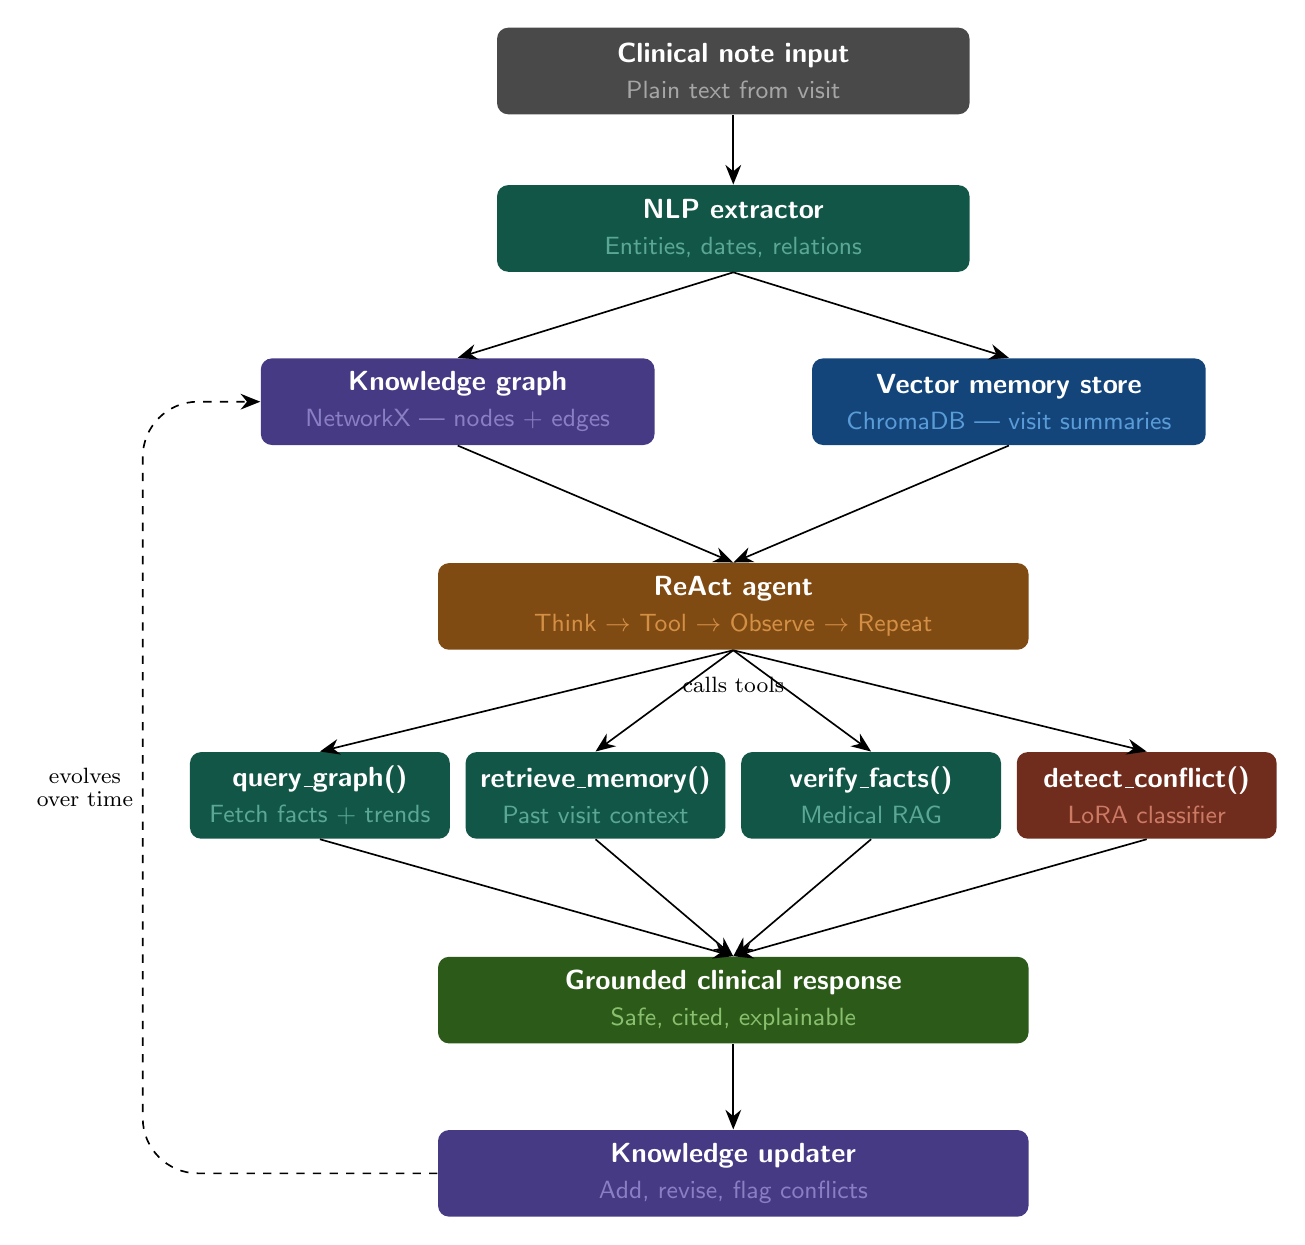
\begin{tikzpicture}[
    font=\sffamily,
    box/.style={rectangle, rounded corners=4pt, align=center, text=white, minimum height=1.1cm}
]

% Level 1
\node[box, fill=cinput, minimum width=6cm] (input) at (0, 0) {
    \textbf{Clinical note input}\\[1pt]
    \textcolor{gray!70}{\small Plain text from visit}
};

% Level 2
\node[box, fill=cnlp, minimum width=6cm] (nlp) at (0, -2) {
    \textbf{NLP extractor}\\[1pt]
    \textcolor{t_nlp}{\small Entities, dates, relations}
};

% Level 3
\node[box, fill=cgraph, minimum width=5cm] (graph) at (-3.5, -4.2) {
    \textbf{Knowledge graph}\\[1pt]
    \textcolor{t_graph}{\small NetworkX --- nodes + edges}
};

\node[box, fill=cvector, minimum width=5cm] (vector) at (3.5, -4.2) {
    \textbf{Vector memory store}\\[1pt]
    \textcolor{t_vector}{\small ChromaDB --- visit summaries}
};

% Level 4
\node[box, fill=cagent, minimum width=7.5cm] (agent) at (0, -6.8) {
    \textbf{ReAct agent}\\[1pt]
    \textcolor{t_agent}{\small Think $\rightarrow$ Tool $\rightarrow$ Observe $\rightarrow$ Repeat}
};

% Annotation
\node[text=black, font=\footnotesize] at (0, -7.8) {calls tools};

% Level 5 (Tools)
\node[box, fill=cnlp, minimum width=3.3cm] (tool1) at (-5.25, -9.2) {
    \textbf{query\_graph()}\\[1pt]
    \textcolor{t_nlp}{\small Fetch facts + trends}
};

\node[box, fill=cnlp, minimum width=3.3cm] (tool2) at (-1.75, -9.2) {
    \textbf{retrieve\_memory()}\\[1pt]
    \textcolor{t_nlp}{\small Past visit context}
};

\node[box, fill=cnlp, minimum width=3.3cm] (tool3) at (1.75, -9.2) {
    \textbf{verify\_facts()}\\[1pt]
    \textcolor{t_nlp}{\small Medical RAG}
};

\node[box, fill=clora, minimum width=3.3cm] (tool4) at (5.25, -9.2) {
    \textbf{detect\_conflict()}\\[1pt]
    \textcolor{t_lora}{\small LoRA classifier}
};

% Level 6
\node[box, fill=coutput, minimum width=7.5cm] (output) at (0, -11.8) {
    \textbf{Grounded clinical response}\\[1pt]
    \textcolor{t_output}{\small Safe, cited, explainable}
};

% Level 7
\node[box, fill=cgraph, minimum width=7.5cm] (updater) at (0, -14.0) {
    \textbf{Knowledge updater}\\[1pt]
    \textcolor{t_graph}{\small Add, revise, flag conflicts}
};

% Arrows
\begin{scope}[every path/.style={-{Stealth[length=2.5mm, width=2mm]}, black, semithick}]
    \draw (input.south) -- (nlp.north);
    \draw (nlp.south) -- (graph.north);
    \draw (nlp.south) -- (vector.north);
    \draw (graph.south) -- (agent.north);
    \draw (vector.south) -- (agent.north);

    \draw (agent.south) -- (tool1.north);
    \draw (agent.south) -- (tool2.north);
    \draw (agent.south) -- (tool3.north);
    \draw (agent.south) -- (tool4.north);

    \draw (tool1.south) -- (output.north);
    \draw (tool2.south) -- (output.north);
    \draw (tool3.south) -- (output.north);
    \draw (tool4.south) -- (output.north);

    \draw (output.south) -- (updater.north);
\end{scope}

% Feedback loop
\draw[-{Stealth[length=2.5mm, width=2mm]}, black, semithick, dashed, rounded corners=20pt]
    (updater.west) -- (-7.5, -14.0) -- (-7.5, -4.2) -- (graph.west);
\node[left, text=black, font=\footnotesize, align=center] at (-7.5, -9.1) {evolves\\[-1pt]over time};

\end{tikzpicture}%
}
\caption{System architecture overview with five components and data flow.}
\label{fig:architecture}
\end{figure*}

\section{Implementation}
This section describes implementation details of the GraphMed pipeline.

\subsection{Pipeline Components and Data Artifacts}
The implementation begins with clinical text processing to convert raw patient files into structured extracted visits. It then constructs and validates temporal graphs, builds vector memory stores, and populates a medical knowledge base for grounded lookups. The runtime layer executes the interactive agent, while a dedicated training workflow generates contradiction data and trains a LoRA classifier. A final testing workflow validates graph evolution and conflict handling scenarios.

Primary artifacts include processed patient files, graph JSON files, vector index directories, medical KB assets, trained model checkpoints, and training metadata. This artifact-first structure enables independent replay of each component and supports selective reprocessing when one stage is updated.

\subsection{Patient Graph Schema}
The patient graph schema represents entities as typed nodes (condition, medication, symptom, lab, visit) and connects them with temporal and semantic edges. Visit nodes anchor chronology and allow first versus latest evidence extraction. Entity nodes maintain confidence and update metadata to support decay and conflict aware maintenance. A simplified schema is:
\begin{itemize}
    \item Node attributes: type, canonical name, confidence, first seen visit, latest seen visit.
    \item Edge attributes: relation type, source visit, timestamp, confidence, operation tag.
    \item Update operations: ADD, UPDATE, CONFLICT.
\end{itemize}

\subsection{ReAct Tools and Execution Flow}
For each question, the agent performs intent aware routing, retrieves candidate evidence from graph and memory, executes safety or conflict checks as needed, and then composes the final answer. Tool invocations are logged for debugging and evaluation traceability.

\begin{table}[t]
\caption{Implementation Stack}
\label{tab:stack}
\centering
\begin{tabular}{p{0.19\linewidth}p{0.24\linewidth}p{0.48\linewidth}}
\toprule
Component & Technology & Role in Pipeline \\
\midrule
NLP Extraction & Python + rule patterns + optional LLM & Visit level entity and relation extraction \\
Temporal Graph & NetworkX + JSON persistence & Per patient evolving KG storage and updates \\
Vector Memory & Chroma vector DB & Semantic retrieval over visit narratives \\
Clinical KB & Curated local corpus + API retrieval hooks & Grounding for drug and condition queries \\
Agent Runtime & ReAct style orchestrator & Tool planning, evidence aggregation, response synthesis \\
Conflict Model & BERT + PEFT LoRA & Binary CONSISTENT vs CONFLICT classification \\
Evaluation Harness & Evaluation scripts + CSV/JSON outputs & Reproducible metrics and audit artifacts \\
\bottomrule
\end{tabular}
\end{table}

\subsection{LoRA Conflict Classifier Configuration}
The conflict classifier is trained on synthetic pairwise statements with balanced labels and evaluates binary contradiction detection. The training metadata in the repository reports perfect test performance on the synthetic split, which is strong but requires cautious interpretation for real world generalization.

\begin{table}[t]
\caption{LoRA Training Configuration}
\label{tab:lora}
\centering
\begin{tabular}{p{0.45\linewidth}p{0.45\linewidth}}
\toprule
Setting & Value \\
\midrule
Base model & google-bert/bert-base-uncased \\
Task type & Sequence classification (binary) \\
LoRA rank ($r$) & 8 \\
LoRA alpha & 16 \\
LoRA dropout & 0.1 \\
Target modules & query, key, value \\
Epochs & 3 \\
Learning rate & $3 \times 10^{-5}$ \\
Batch size & 16 \\
Train/Val/Test sizes & 6400 / 800 / 800 \\
Reported test metrics & Accuracy 1.0, F1 1.0, Precision 1.0, Recall 1.0 \\
\bottomrule
\end{tabular}
\end{table}

\begin{figure}[t]
\centering
\resizebox{0.46\textwidth}{!}{%
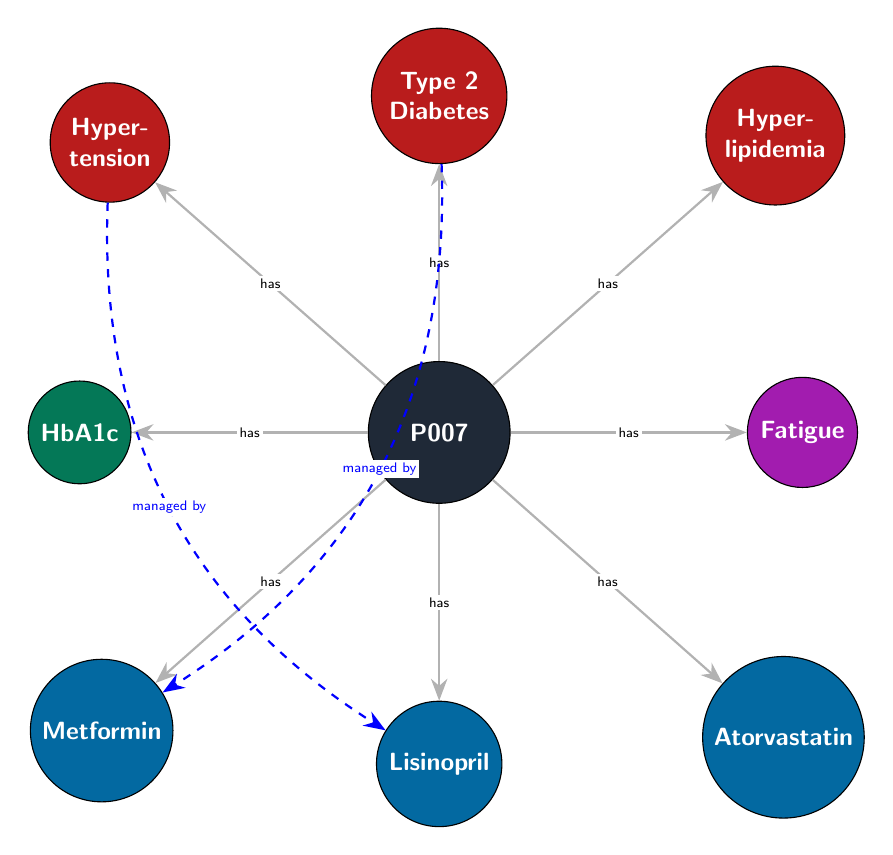
\begin{tikzpicture}[
    node distance=2.5cm and 3cm,
    base/.style={circle, draw, minimum size=1.2cm, font=\sffamily\small\bfseries, align=center, text=white},
    patient/.style={base, fill=patientColor, minimum size=1.8cm},
    condition/.style={base, fill=conditionColor},
    medication/.style={base, fill=medicationColor},
    lab/.style={base, fill=labColor},
    symptom/.style={base, fill=symptomColor},
    has/.style={-{Stealth[scale=1.2]}, thick, draw=gray!60},
    labelStyle/.style={font=\sffamily\tiny, fill=white, inner sep=1pt}
]

\node[patient] (P007) {P007};

\node[condition, above=of P007] (T2D) {Type 2\\Diabetes};
\node[condition, above left=of P007] (HTN) {Hyper-\\tension};
\node[condition, above right=of P007] (HLD) {Hyper-\\lipidemia};

\node[medication, below left=of P007] (Met) {Metformin};
\node[medication, below=of P007] (Lis) {Lisinopril};
\node[medication, below right=of P007] (Ato) {Atorvastatin};

\node[lab, left=of P007] (HbA1c) {HbA1c};
\node[symptom, right=of P007] (Fatigue) {Fatigue};

\draw[has] (P007) -- (HTN) node[midway, labelStyle] {has};
\draw[has] (P007) -- (T2D) node[midway, labelStyle] {has};
\draw[has] (P007) -- (HLD) node[midway, labelStyle] {has};
\draw[has] (P007) -- (Met) node[midway, labelStyle] {has};
\draw[has] (P007) -- (Lis) node[midway, labelStyle] {has};
\draw[has] (P007) -- (Ato) node[midway, labelStyle] {has};
\draw[has] (P007) -- (HbA1c) node[midway, labelStyle] {has};
\draw[has] (P007) -- (Fatigue) node[midway, labelStyle] {has};

\draw[has, dashed, blue] (HTN) to [bend right] node[midway, labelStyle] {managed by} (Lis);
\draw[has, dashed, blue] (T2D) to [bend left] node[midway, labelStyle] {managed by} (Met);

\end{tikzpicture}%
}
\caption{Example temporal patient graph after three visits.}
\label{fig:kg}
\end{figure}

\section{Experiments and Results}
\subsection{Evaluation Setup}
The Phase 9 evaluation harness compares GraphMed and a baseline RAG system without graph based memory evolution or contradiction handling. Three experiments are executed: E1 factual QA, E2 longitudinal memory consistency, and E3 conflict detection. Results are exported to JSON and CSV for reproducibility.

E1 uses 50 patient scoped questions generated from processed records, spanning history, multi visit context, drug safety, and lab trend prompts. E2 evaluates longitudinal behavior on 50 cases using similarity and consistency proxies. E3 injects 30 contradiction cases and measures binary detection quality. Runtime mode is full stack with provider routing configured through environment variables.

\subsection{Experiment 1: Factual QA}
E1 reports mean FactScore computed via expected keyword coverage after normalization. Overall factual QA favors baseline in this run (0.6533 vs 0.5533), but the multi visit subset favors GraphMed (0.6333 vs 0.5000), supporting the claim that graph grounded memory helps temporal context questions.

\subsection{Experiment 2: Longitudinal Consistency}
E2 currently underperforms baseline on both reported proxies in this snapshot. GraphMed records BERTScore mean of -0.1339 and consistency mean of -0.0127, while baseline records 0.0580 and 0.1843, respectively. This identifies a concrete optimization target in answer normalization and temporal summarization policy.

\subsection{Experiment 3: Conflict Detection}
E3 is the strongest result in the current run. GraphMed obtains precision, recall, and F1 of 1.0 each, while baseline and the fallback prompt only comparator register 0.0 across the same metrics. This behavior aligns with the dedicated LoRA contradiction model and explicit conflict aware tooling.

\begin{table}[t]
\caption{Main Experimental Results (Phase 9 Snapshot)}
\label{tab:main_results}
\centering
\begin{tabular}{p{0.38\linewidth}p{0.22\linewidth}p{0.22\linewidth}}
\toprule
Metric & GraphMed & Baseline \\
\midrule
E1 FactScore mean (50) & 0.5533 & 0.6533 \\
E1 Multi-visit FactScore mean & 0.6333 & 0.5000 \\
E2 BERTScore mean (50) & -0.1339 & 0.0580 \\
E2 Consistency mean (50) & -0.0127 & 0.1843 \\
E3 Precision (30) & 1.0000 & 0.0000 \\
E3 Recall (30) & 1.0000 & 0.0000 \\
E3 F1 (30) & 1.0000 & 0.0000 \\
\bottomrule
\end{tabular}
\end{table}

\begin{figure}[t]
\centering
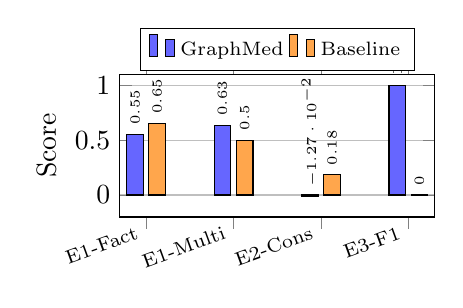
\begin{tikzpicture}
\begin{axis}[
    ybar,
    bar width=6pt,
    width=0.46\textwidth,
    height=0.28\textwidth,
    ylabel={Score},
    symbolic x coords={E1-Fact,E1-Multi,E2-Cons,E3-F1},
    xtick=data,
    x tick label style={font=\scriptsize, rotate=20, anchor=east},
    ymajorgrids=true,
    ymin=-0.2,
    ymax=1.1,
    legend style={font=\scriptsize, at={(0.5,1.02)}, anchor=south, legend columns=2},
    nodes near coords,
    every node near coord/.append style={font=\tiny, rotate=90, anchor=west}
]
\addplot[fill=blue!60] coordinates {
    (E1-Fact,0.5533)
    (E1-Multi,0.6333)
    (E2-Cons,-0.0127)
    (E3-F1,1.0000)
};
\addplot[fill=orange!70] coordinates {
    (E1-Fact,0.6533)
    (E1-Multi,0.5000)
    (E2-Cons,0.1843)
    (E3-F1,0.0000)
};
\legend{GraphMed,Baseline}
\end{axis}
\end{tikzpicture}
\caption{Cross experiment metric comparison.}
\label{fig:bars}
\end{figure}

\subsection{Ablation Study Protocol and Current Status}
An ablation comparison is required to validate contribution attribution. The protocol below isolates graph memory, vector memory, and LoRA classifier effects. In the current repository snapshot, complete ablation runs were not yet exported alongside main Phase 9 artifacts, so the table reports available values and marks pending rows for execution.

\subsection{Evaluation Driven Updates}
A notable operational result is closed loop maintenance: evaluation flagged 11 patients and applied 21 update events in an automated pass. This indicates that the system can use performance signals not only for reporting but also for targeted graph refinement.

\section{Discussion}
The current results show a mixed but informative profile. GraphMed clearly excels at contradiction detection and improves multi visit factual QA relative to baseline, yet underperforms on the present E2 longitudinal consistency proxies. This suggests the architecture is directionally correct for safety critical conflict handling but requires refinement in how temporal evidence is compressed into final answers.

Several limitations are important. First, data realism: synthetic generation and transformed timelines may not capture the lexical noise, coding variability, and rare events seen in production EHRs. Second, domain scope: MIMIC aligned data tends to reflect ICU centered workflows, while many medication management problems are outpatient and chronic care heavy. Third, integration scope: the current pipeline is file and batch oriented rather than real time EHR event streaming.

Threats to validity include potential leakage between generated training templates and evaluation phrasing, especially for conflict detection where synthetic patterns may be easier than naturally occurring contradictions. Another threat is metric coupling: keyword based factual scoring can reward lexical overlap even when clinical framing differs, and can penalize semantically valid paraphrases if normalization is insufficient. Also, perfect synthetic conflict metrics should be interpreted as internal feasibility, not definitive clinical readiness.

From a systems perspective, reproducibility is a strength. Phase based scripts, deterministic settings, and JSON/CSV artifact export make regression checks straightforward. However, robustness to provider rate limits, model drift, and extraction errors remains an active engineering concern. A practical next step is to complete the ablation grid and re run E2 with revised temporal summarization constraints to determine whether consistency underperformance is metric specific or architectural.

\section{Conclusion}
This paper presented GraphMed, a longitudinal clinical reasoning framework that combines temporal patient knowledge graphs, GraphRAG retrieval, a ReAct tool orchestrator, and a LoRA based contradiction classifier. The implementation is structured as a modular phase pipeline and evaluated with reproducible artifact export across three experiments.

Empirically, the current Phase 9 snapshot demonstrates strong contradiction handling (E3 F1 of 1.0 versus 0.0 baseline) and improved multi visit factual behavior in E1 (0.6333 versus 0.5000 on the multi visit subset), while highlighting a clear weakness in E2 longitudinal consistency proxies that requires targeted optimization. This combination of strengths and deficits provides a concrete roadmap: preserve the conflict safety gains while improving temporal synthesis quality.

Future work will focus on three directions. First, data and evaluation expansion: execute full ablation runs, add clinician written longitudinal queries, and include external validation cohorts. Second, deployment realism: move from batch files to secure real time EHR streaming with stronger audit trails. Third, modeling breadth: extend beyond text with multimodal signals such as imaging summaries and waveform trends, and investigate privacy preserving federated adaptation for hospital specific fine tuning.

\section*{References}

\begin{thebibliography}{00}
\bibitem{b1} X. Liang and Z. Gu, "Fast Think-on-Graph: Wider, Deeper and Faster Reasoning of Large Language Model on Knowledge Graph," arXiv preprint arXiv:2501.14300, 2025.

\bibitem{b2} J. Lin, S. Wang, X. Guo, J. Shun, and Y. Zhu, "Temporal Reasoning over Evolving Knowledge Graphs," arXiv preprint arXiv:2509.15464, 2025.

\bibitem{b3} J. Wang, K. Sun, L. Luo, W. Wei, Y. Hu, A. W.-C. Liew, S. Pan, and B. Yin, "Large Language Models-guided Dynamic Adaptation for Temporal Knowledge Graph Reasoning," NeurIPS, 2024.

\bibitem{b4} P. Lewis \textit{et al.}, "Retrieval-Augmented Generation for Knowledge-Intensive NLP Tasks," NeurIPS, 2020.

\bibitem{b5} J. Wei \textit{et al.}, "Chain-of-Thought Prompting Elicits Reasoning in Large Language Models," arXiv, 2022.

\bibitem{b6} D. Edge \textit{et al.}, "From Local to Global: A Graph RAG Approach to Query-Focused Summarization," arXiv, 2024.

\bibitem{b7} D. Vrandecic and M. Krotzsch, "Wikidata: A Free Collaborative Knowledge Base," \textit{Communications of the ACM}, 2014.

\end{thebibliography}

\end{document}
